We designed and implemented the algorithm to be used by robots in real-world missions and applications. Therefore, real-world experiments played a vital role in ensuring our algorithm's implementation can perform in the real world. For this reason, multiple experiments were conducted to test the performance of our algorithm.\\
The experiments were conducted in a controlled environment, with the robot crossing the road at a pre-defined location. For our experiments, we used the robot Spot from Boston Dynamics. As the detection node was not a part of this thesis and was not finished when the experiments took place, we had to use a different method to simulate the detection of vehicles.

\section{Simulation of vehicle detection node}
    For simulating the detection of vehicles, we opted to use a detector of AprilTags. AprilTags are a type of fiducial markers that are used for localization and pose estimation. They are specifically designed to be easily detectable by cameras. We used the \texttt{tag16h5} family, and the tag used to represent the vehicle is shown in figure \ref{fig:apriltag}.\\
    \begin{figure}[ht]
        \centering
        
\includegraphics[trim={1 1 1 1}, clip, width=0.3\textwidth]{images/tag16_05_00007.png}
        \caption{AprilTag used for simulating the detection of vehicles.}
        \label{fig:apriltag}
    \end{figure}
    For the detection of the AprilTag, we used the \textit{apriltag\_ros} package\footnote{\url{https://github.com/AprilRobotics/apriltag_ros}}. This package provides a ROS node, which subscribes to the image topic and publishes the pose of the detected AprilTags. A node to convert the pose from the camera frame to the body frame of the robot was also implemented. This node's other task was to take the transformed pose and convert it to the vehicle information necessary for our algorithm. The calculation of the velocity and acceleration of the vehicle was done only from the current and previous measurements.

\section{Experimental setup}
    The experiment was conducted in the courtyard of our faculty. The robot was placed at the edge of the sidewalk, which served the purpose of a road the robot should cross. The map of the experimental area with the initial position of the robot is shown in figure \ref{fig:map}.\\
    \begin{figure}[ht]
        \centering
        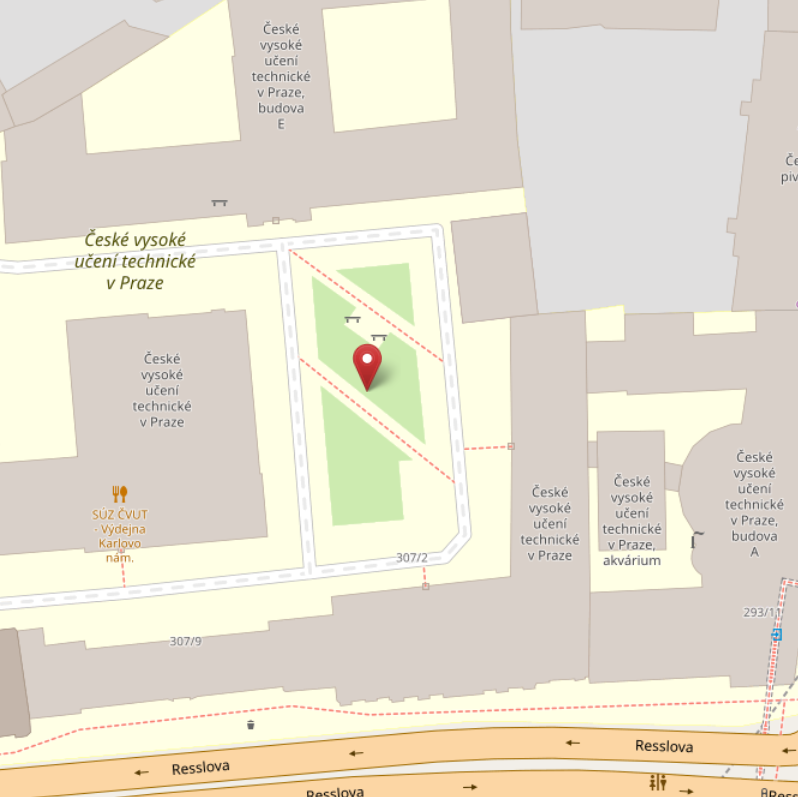
\includegraphics[width=0.8\textwidth]{images/map.png}
        \caption{Map of the experimental area taken from OSM.}
        \label{fig:map}
    \end{figure}
    In experiments containing the detection of vehicles, the AprilTag was carried by the thesis supervisor alongside the road.\\
    For all experimental setups, the width of the road was set to $6\:\si{\m}$. And the width and length of the detected vehicle were set to $1\:\si{\m}$ and $2\:\si{\m}$ respectively.\\
    The maximal number of vehicles in the experiments was set to 1. This was done to simplify the experiments, as the detection of multiple AprilTags would require a more complex setup.

\section{Conducted experiments}
    Due to the limited time and resources, we could only conduct a limited number of experiments. The experiments were conducted in two phases. In the first phase, we tested the algorithm without any vehicles present. In the second phase, the vehicles were introduced into the environment.

    \subsection{Experiments without vehicles}
        The first phase was designed to test the algorithm without any vehicles present. The goal of this phase was to ensure that the robot could cross the road, meaning that the algorithm was able to control the movement of the robot.\\
        As a part of the algorithm where the robot is being positioned perpendicular to the road could not be tested in simulations, we tested it extensively as a part of this experiment. We were unable to test it in the simulation experiments as the simulation of the magnetometer was not functional.\\\\
        \bfc{Results}\\
            We started with the robot angled away from the ideal position, figure \ref{fig:init1}. The robot was able to rotate itself to reach the ideal perpendicular position, figure \ref{fig:perpendicular}. After reaching the perpendicular position, the robot was able to cross the road and stop at the other side, figure \ref{fig:final1}.\\
            \begin{figure}[ht]
                \centering
                \begin{subfigure}{0.49\textwidth}
                    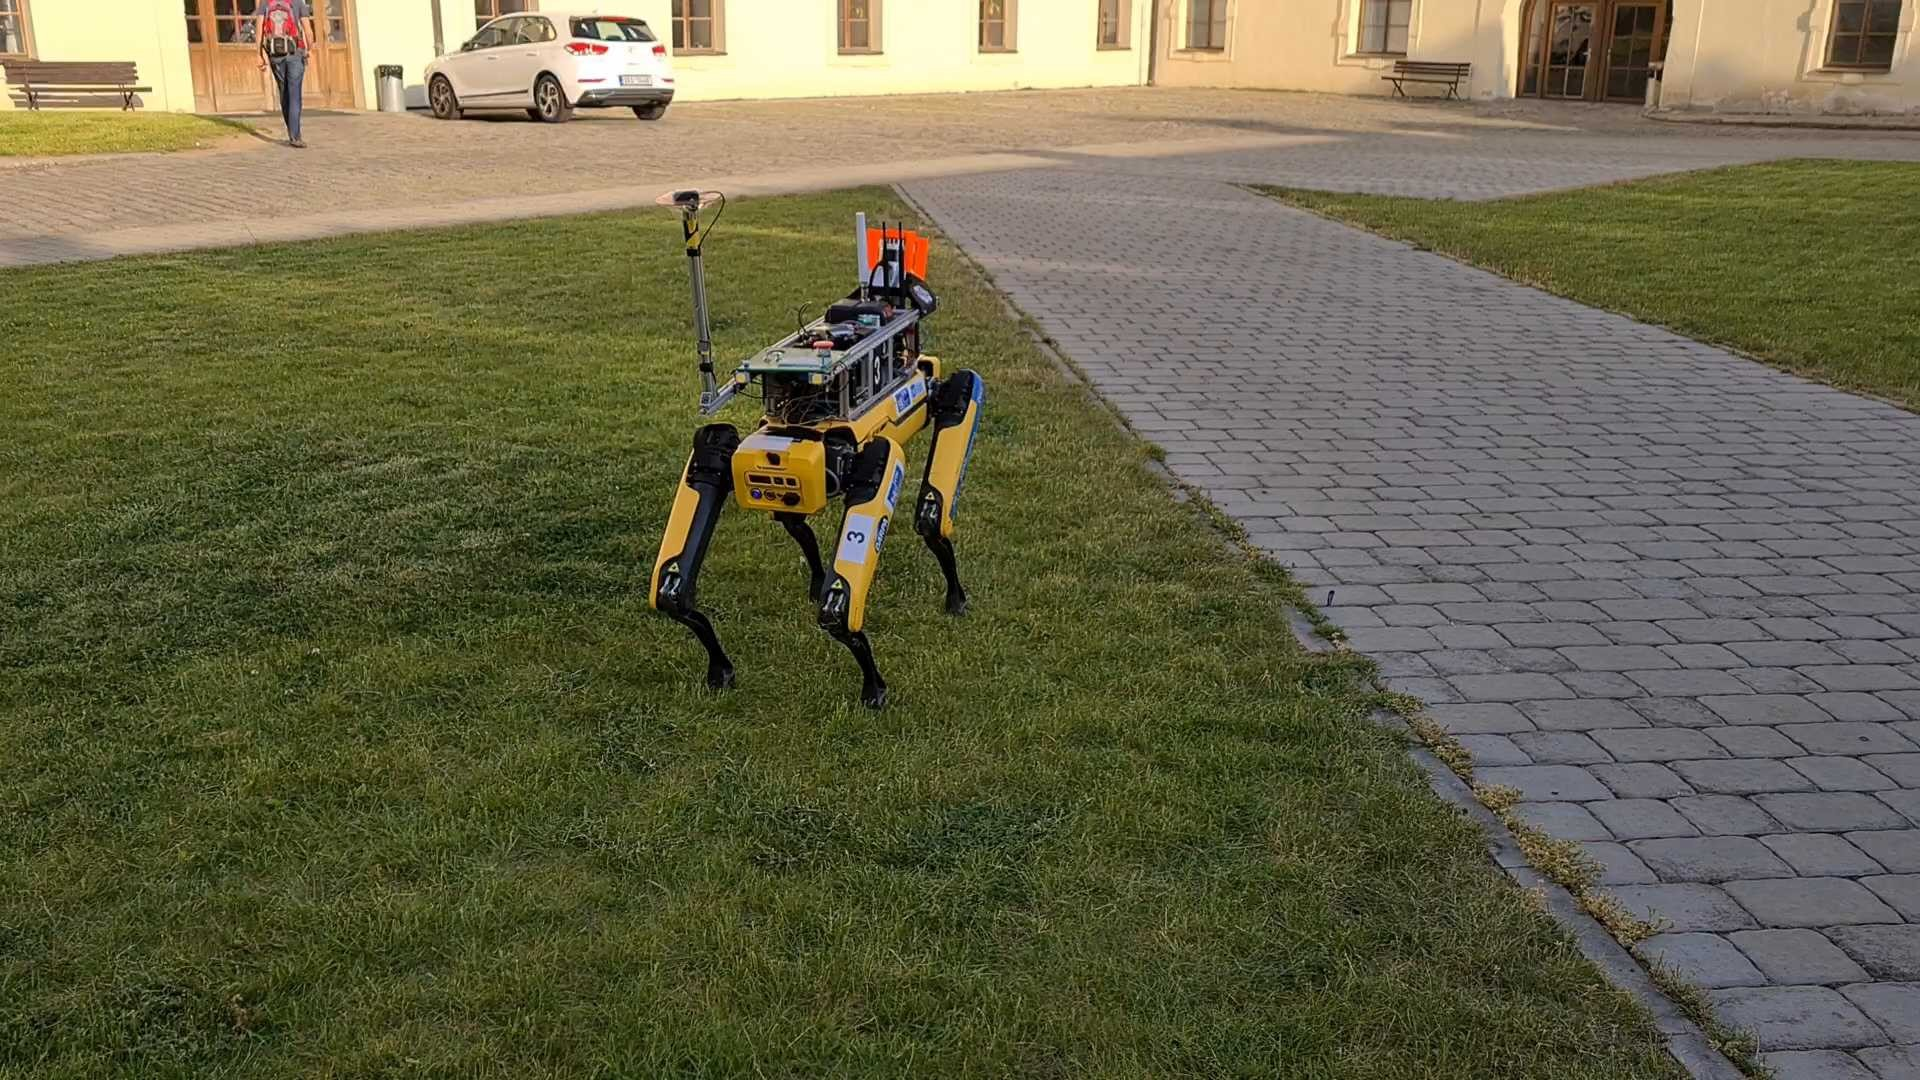
\includegraphics[width=\textwidth]{images/init1.jpg}
                    \caption{Initial position.}
                    \label{fig:init1}
                \end{subfigure}
                \begin{subfigure}{0.49\textwidth}
                    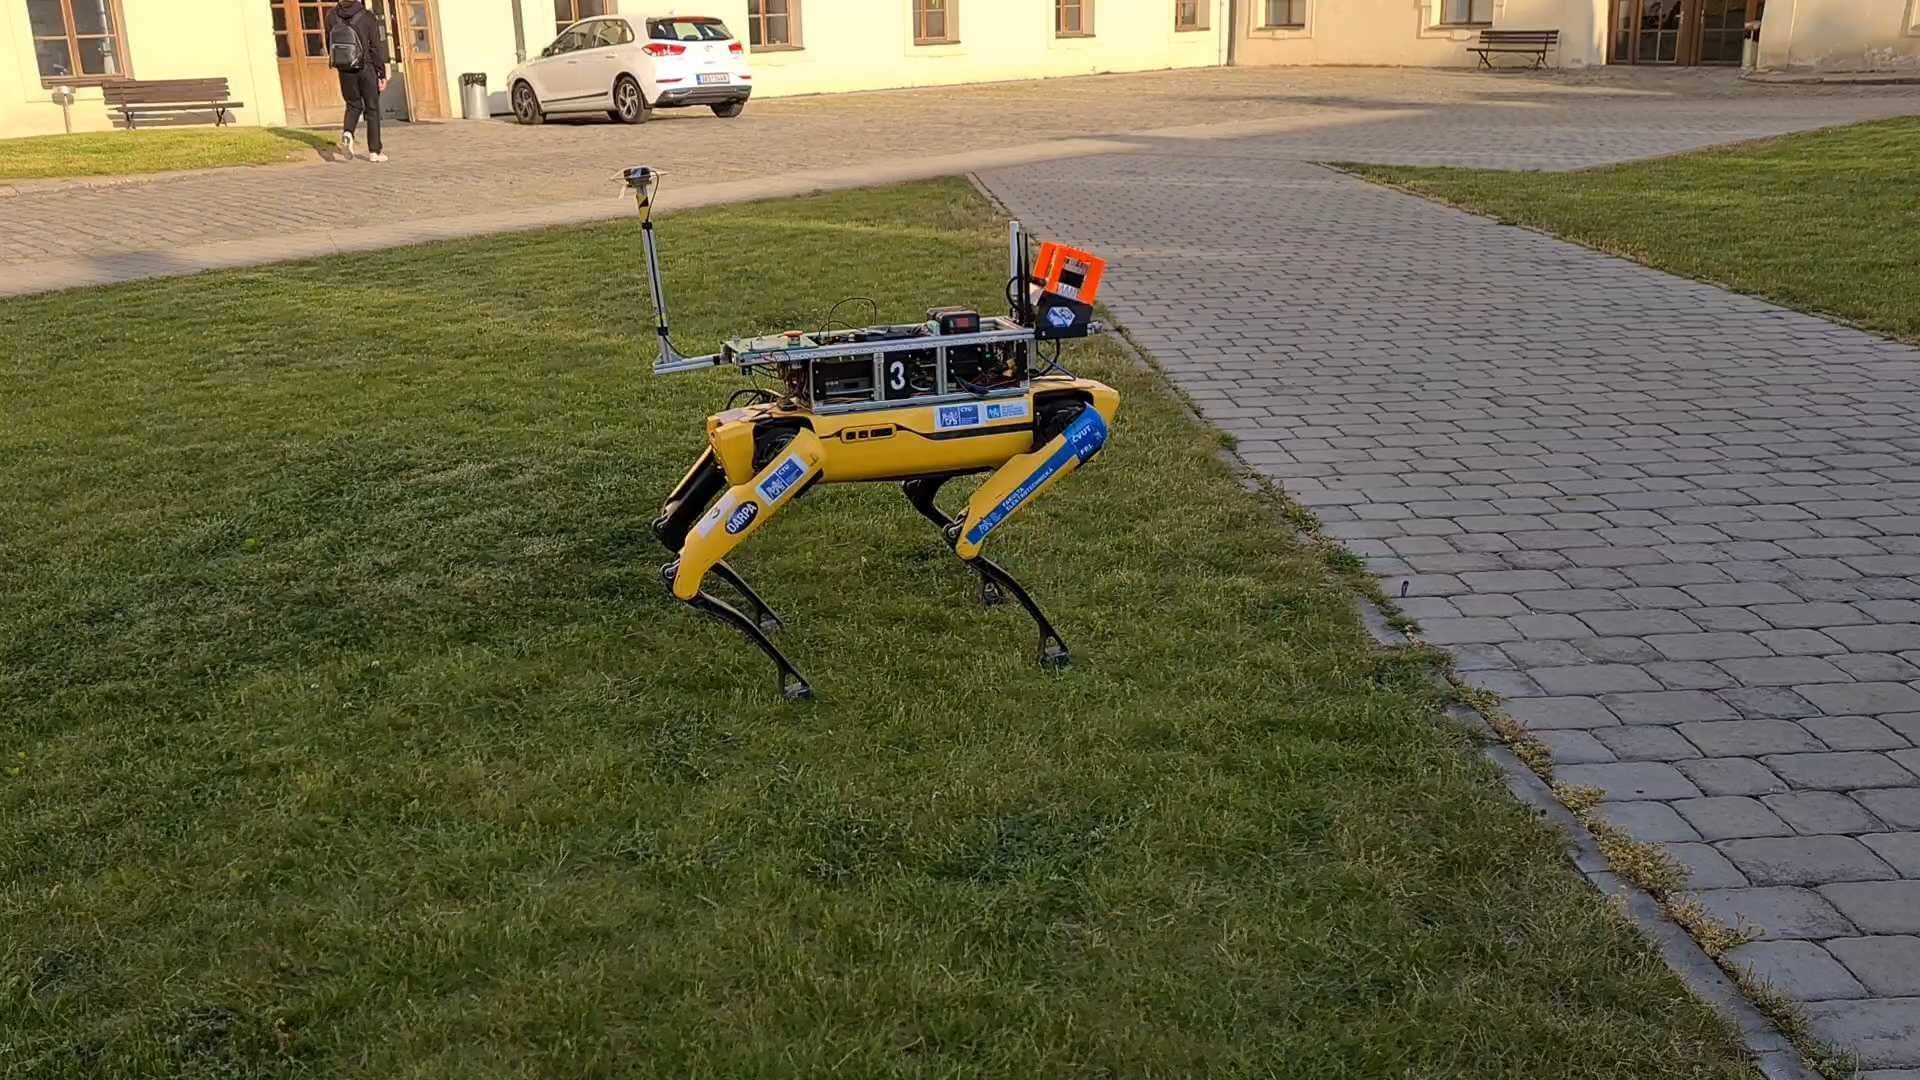
\includegraphics[width=\textwidth]{images/perpendicular.jpg}
                    \caption{Perpendicular position.}
                    \label{fig:perpendicular}
                \end{subfigure}
                \begin{subfigure}{0.49\textwidth}
                    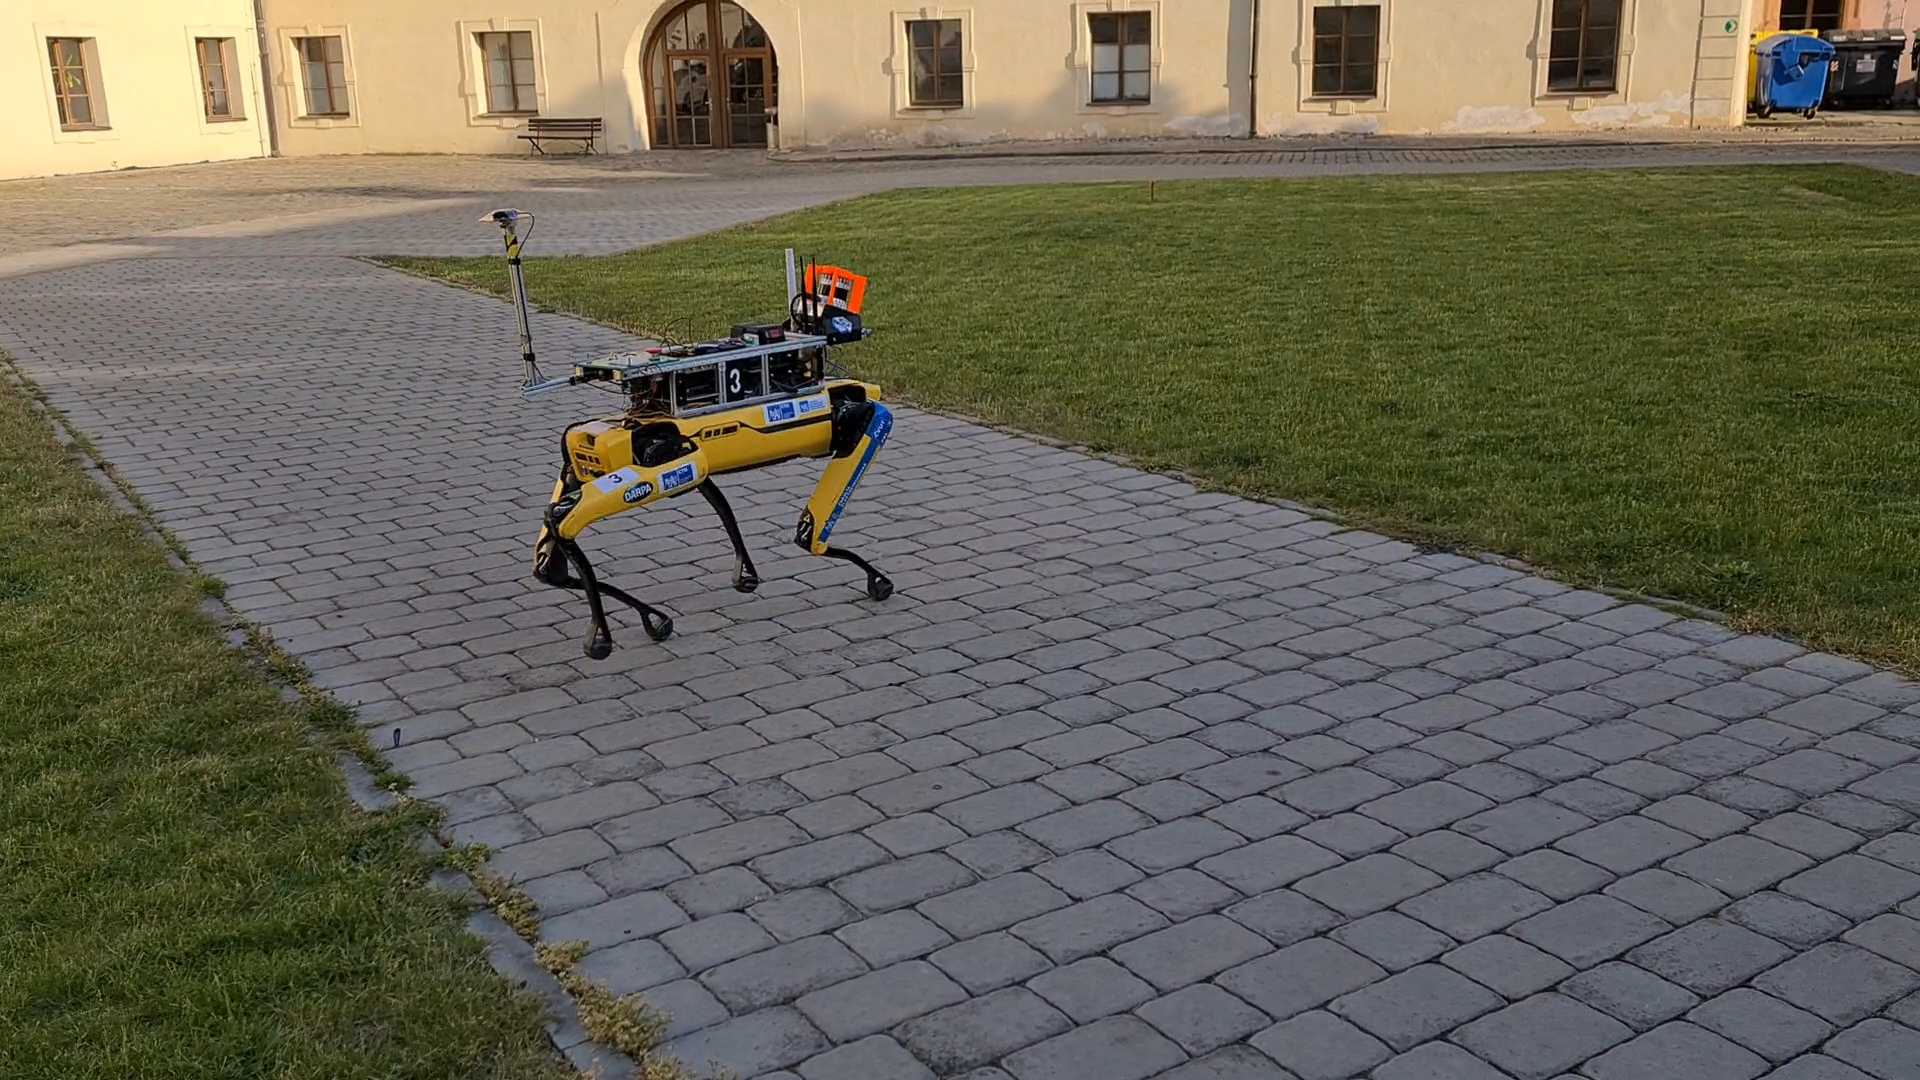
\includegraphics[width=\textwidth]{images/during1.jpg}
                    \caption{Robot during the crossing.}
                \end{subfigure}
                \begin{subfigure}{0.49\textwidth}
                    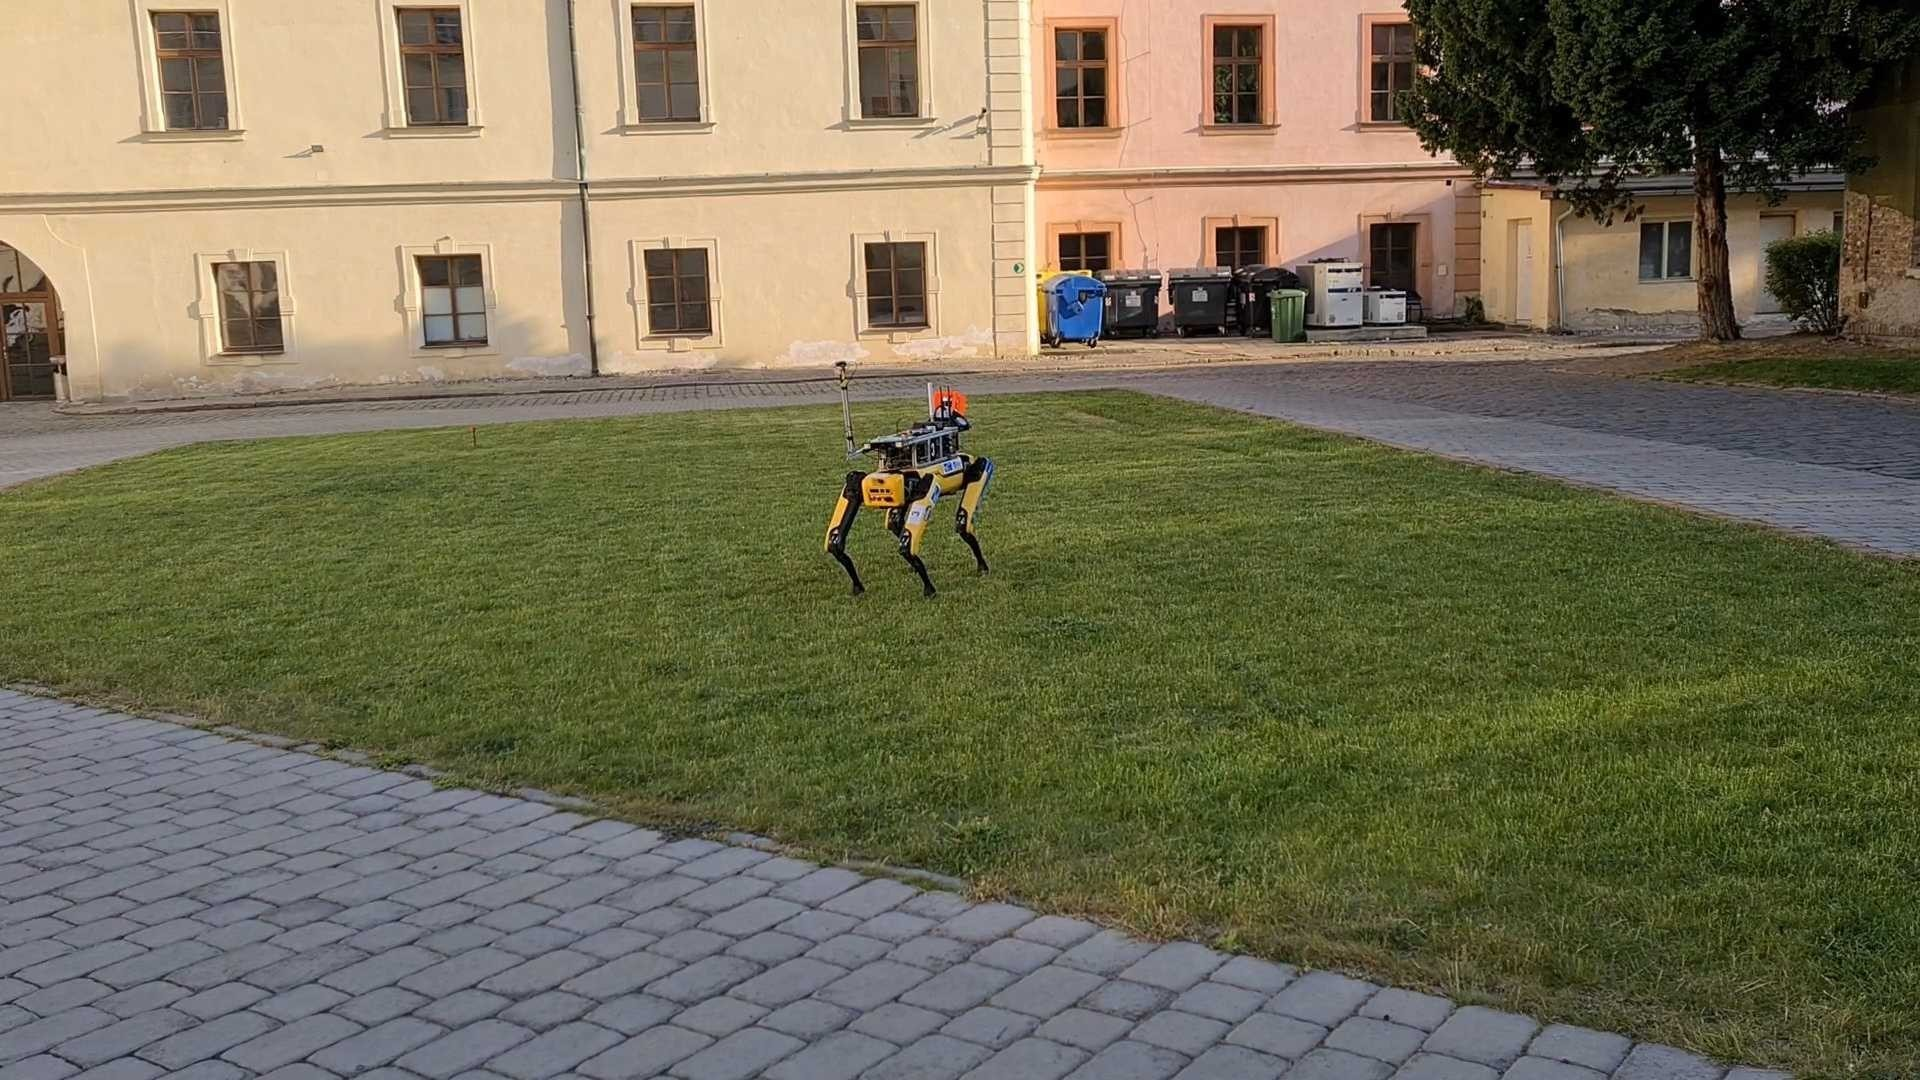
\includegraphics[width=\textwidth]{images/final1.jpg}
                    \caption{Final position.}
                    \label{fig:final1}
                \end{subfigure}
                \caption{Photos from the experiment without vehicles.}
            \end{figure}
            The algorithm successfully determined the correct azimuth for the robot and rotated it to reach the position. The robot was able to cross the road and evaluate its position to determine that it had reached the other side.

    \subsection{Experiments with vehicles}
        In the second phase, we tested the algorithm with vehicles present. The goal of this phase was to test the algorithm in a more realistic scenario. We wanted to test the decision-making of the algorithm with real-world data from the detection node.\\
        These experiments were more challenging as we had to troubleshoot the detection node, which was not a part of this thesis. We were able to conduct only one successful experiment with the detection node, as the detection node could not consistently detect the AprilTag in the other experiments. Given the limited time available, fixing the detection node to conduct more experiments was not feasible. We also did not record the successful experiment, as we did not expect it to be the only successful one.

    \subsection{Evaluation of the experiments}
        The experiments were successful in testing the algorithm's ability to use real data. The robot was able to utilize data from GNSS and magnetometer to determine its position and orientation. The robot was also able to process data provided by the detection node to determine the presence and position of vehicles.\\
        Both experiments were successful in testing the algorithm in a real-world environment. The algorithm was able to control the movement of the robot and successfully and safely cross the road.
